\documentclass[]{thesis-ekf}
\usepackage[T1]{fontenc}
\PassOptionsToPackage{defaults=hu-min}{magyar.ldf}
\usepackage{fancyvrb,listingsutf8,xcolor,caption}
\usepackage{fancyhdr,amsthm,amsmath,amssymb,listings}
\usepackage[magyar]{babel}
\lstdefinestyle{user1}{
	inputencoding=utf8/latin2,
	language=[Sharp]C,
	basicstyle=\footnotesize,
	numbers=left,
	xleftmargin=0.5cm,
	xrightmargin=0.5cm,
	breaklines,
	postbreak=\hbox{$\color{red}\hookrightarrow\ $},
	backgroundcolor=\color{gray!20},
	frame=tblr,
	framesep=3pt,
	keywordstyle=\bfseries\color{blue},
	commentstyle=\itshape\color{teal},
}
\lstdefinestyle{user2}{
	inputencoding=utf8/latin2,
	language=C++,
	basicstyle=\footnotesize,
	numbers=left,
	xleftmargin=0.5cm,
	xrightmargin=0.5cm,
	breaklines,
	postbreak=\hbox{$\color{red}\hookrightarrow\ $},
	backgroundcolor=\color{gray!20},
	frame=tblr,
	framesep=3pt,
	keywordstyle=\bfseries\color{blue},
	commentstyle=\itshape\color{teal},
}
\theoremstyle{definition}
\newtheorem{definicio}{Definíció}[chapter]
\DeclareMathOperator{\tg}{tg}
\setlength{\headheight}{15pt}
\renewcommand{\lstlistingname}{kód}


\begin{document}
	\institute{Természettudományi Kar - TTK}
	\title{Objektumorientált programozás}
	\author{Csongrádi Ferenc Péter\\Programtervező informatikus Bsc}
	\supervisor{Dr. Tómács Tibor\\Egyetemi Docens}
	\city{Eger}
	\date{2020}
	
	\maketitle
	\tableofcontents
	\chapter{Bevezető}
	Az objektumorientált vagy objektumelvű programozás\footnote{angolul object-oriented programming, röviden OOP} az objektumok fogalmán alapuló \emph{programozási paradigma}. (lásd \az{\ref{paradigma}}.~definíció.) Az objektumok egységbe foglalják az adatokat és a hozzájuk tartozó műveleteket. Az adatokat ismerik mezők, attribútumok, tulajdonságok néven, a műveleteket metódusokként szokták emlegetni. Az objektum által tartalmazott adatokon általában az objektum metódusai végeznek műveletet. A program egymással kommunikáló objektumok összességéből áll.\cite{Kindler2011} A legtöbb objektumorientált nyelv osztály alapú, azaz az objektumok osztályok példányai, és típusuk az osztály.
	
	Például egy hétköznapi fogalom, a ,,kutya'' felfogható egy osztály (a kutyák osztálya) tagjaként, annak egyik objektumaként. Minden kutya objektum rendelkezik a kutyákra jellemző tulajdonságokkal (például szőrszín, méret stb.) és cselekvési képességekkel (például futás, ugatás).
	
	A legtöbb széles körben alkalmazott nyelv többek között az objektumorientált programozást is támogatja, tipikusan az imperatív, procedurális programozással együtt. A legfontosabb objektumorientált nyelvek: Java, C++, C\#, Python, PHP, Ruby, Perl, Object Pascal, Objective-C, Dart, Swift, Scala, Common Lisp, és Smalltalk.
	
	Az \emph{objektumorientált programozásban} használt különböző megközelítésekről  \az{\ref{fejezet-megk}}.~fejezetben	\az{\pageref{fejezet-megk}}.~oldalon olvashat.
	
	\begin{definicio}\label{paradigma}
		A \emph{programozási paradigma} egy osztályozási forma, amely a programozási nyelvek jellemzőin alapul. A nyelvek több paradigmába is sorolhatók.
	\end{definicio}
	
	\chapter{Megközelítések}\label{fejezet-megk}
	
	\section{Analízisszintű gondolkodás}
	
	A szoftver fejlesztésének korai fázisaiban a megvalósítandó rendszer feladatait szeretnénk feltérképezni: a funkcionális és egyéb jellegű követelményeket. Más szóval, a kérdés ilyenkor az, hogy a rendszernek mit kellene tennie. Ilyenkor határozzuk meg a szoftver (formális és informális) specifikációját, majd abból kiindulva kezdjük magasabb szintű absztrakciók segítségével előállítani a rendszer modelljét, amely a konkrét megvalósítás alapját fogja képezni.
	
	\section{Tervezésszintű gondolkodás}
	
	A meglévő modell alapján a szoftver konkrét implementációjához\footnote{megvalósításához} vezető utat tervezzük meg. Ilyenkor arra keressük a választ, hogy a meghatározott specifikációt hogyan valósítsa meg a rendszer. -- Ehhez hasznos lehet \az{\eqref{equation}} egyenlet. -- Ezen a szinten már képbe kerülnek különböző alacsony szintű technikák is, mint például a kommunikációs protokollok, programozási nyelvek és technológiák.
	
	\begin{equation}\label{equation}
		f\colon\mathbb{R}\setminus\left\{(2k+1)\frac{\pi}{2}:k\in\mathbb{Z}\right\}
		\to\mathbb{R},\quad f(x):=
		\begin{cases}
			\frac{\tg(x)\sin(x)}{(x+1)},&\text{ha }x\not=-1,\\
			0,&\text{különben}
		\end{cases}
	\end{equation}
	
	\chapter{Képességek}\label{fejezet-kep}
	
	Az objektumorientált programozás objektumokat használ, de nem minden objektumorientált nyelv támogatja az összes hozzá tartozó technikát és szerkezetet. A továbbiakban felsorolt képességek azonban elterjedtek az erősen osztály-és objektumorientált nyelvek, valamint multiparadigma nyelvek között. Emellett a ritka kivételeket is be fogjuk mutatni.\az{\cite[278.~oldalon]{Mitchell}} \az{\cite[470.~oldalon]{Michael}}
	
	\section{Hasonlóság a szekvenciális nyelvekkel}
	
	\begin{itemize}
		\item Kevés fajta beépített típushoz tartozó változókban tárolnak információt. Ezek lehetnek egész, lebegőpontos típusok, lehetnek karaktertípusok; adatszerkezetek, mint stringek vagy tömbök, listák, hashtáblák, vagy pointerek.
		\item Függvények és eljárások, rutinok, szubrutinok, metódusok, amelyek műveleteket végeznek bemenő paramétereiken, és visszaadhatnak értékeket. A modern programozási nyelvek struktuált vezérlési szerkezeteket tartalmaznak, mint feltételes szerkezetek és ciklusok.
	\end{itemize}
	
	A moduláris programozás támogatja a változók, függvények és eljárások csoportosítását szervezési célokkal. A névterek használata elkülöníti a különböző modulokban levő azonos nevű változókat, függvényeket, eljárásokat.
	
	\section{Objektumok és osztályok}
	Az objektumorientált programozást támogató nyelvek tipikusan öröklődéssel támogatják az újrahasznosítást osztályok vagy prototípusok formájában. Az osztályokat használók két alapfogalmat vezettek be:
	
	\begin{itemize}
		\item Osztályok: az adatformátum és az elérhető metódusok definíciója az adott típus vagy a típushoz tartozó objektumok számára. Az osztályok is tartalmazhatnak adattagokat és metódusokat, amelyek műveleteket végeznek az osztály adattagjain. Összetartozó adatok és függvények, eljárások egysége.
		\item Objektumok: az osztály példányai.
	\end{itemize}
	
	Az objektumok gyakran megfeleltethetők a való élet objektumainak vagy egyedeinek. Például egy rajzolóprogram tartalmazhat olyan objektumokat, mint kör, négyzet vagy menü. Egy online áruházban lehetnek olyan objektumok, mint bevásárlókosár, vásárló és termék.\az{\cite[220.~oldalon]{Booch}} Néha az objektumok absztraktabb entitásoknak felelnek meg, például egy megnyitott fájlnak; vagy egy objektum, ami mértékegységek között vált át.
	
	Az objektumok valamelyik osztály példányai. Például, egy objektum, aminek név mezője ,,Mary'', lehet az Employee\footnote{Alkalmazott} osztály példánya. A függvényeket és eljárásokat az objektumorientált programozásban metódusoknak nevezik, a változókat adattagnak, attribútumnak, mezőnek vagy tulajdonságnak. Az objektumorientált programozás bevezeti a következő kifejezéseket:
	
	\begin{itemize}
		\item Osztályváltozók: az osztályhoz tartoznak, elérhetők az osztályon, de példányokon keresztül is. Minden példány számára ugyanaz.
		\item Példányváltozók vagy attribútumok: az egyedi objektumok jellemzői, minden objektumnak sajátja van.
		\item Tagváltozók: az osztály- és a példányváltozók együttese, amik egy osztályban vannak definiálva.
		\item Osztálymetódusok: osztály szintű metódusok, csak az osztályváltozókhoz és paramétereikhez férhetnek hozzá, példányváltozókhoz nem.
		\item Példánymetódusok: példány szintű metódusok, hozzáférnek az adott példány összes adatához és metódusához, és paramétereik is lehetnek.
	\end{itemize}
	
	Az objektumok hozzáférhetők változókként, de belső szerkezetük van. Absztrakciós szintet adnak, ami elválatsztja a belső és a külső kódot. A külső kód az objektum kliense, ami kérheti bizonyos metódusok végrehajtását az objektumtól, írhatja, olvashatja annak változóit. Sok nyelvben a példányokat közvetve, pointerekkel kezelik; maga az objektum a heap-en vagy a stack-en van.
	
	Az objektumokat az osztályban definiált speciális metódus, konstruktor hozza létre. A program több példányt is létrehozhat egy osztályból, amelyek egymástól függetlenül működnek; így a program ugyanazokat a műveleteket végezheti különböző adathalmazokon.
	
	Az osztályokat használó objektumorientált programozást osztály alapú programozásnak is nevezik, míg a prototípus alapú programozásban nincsenek osztályok. Emiatt analóg, de szignifikánsan különböző terminológiát használnak az objektum és példány definiálására.
	
	Egyes nyelvekben további kombinációs lehetőségek is vannak, mint vonások és mixinek.
	
	\section{Osztály alapú és prototípus alapú}
	Osztály alapú nyelvekben az osztályokat előre kell definiálni, az objektumokat ezekből példányosítással kapjuk. Ha az apple\footnote{alma} és orange\footnote{narancs} alapvetően gyümölcsök, a Fruit osztály példányai, ami garantálja, hogy ugyanúgy kezelhetők, például a szín, a cukortartalom vagy az, hogy érett-e.
	
	Prototípus alapú nyelvekben az objektumok elsődleges entitások. Osztályok nincsenek. Ehelyett az objektumoknak prototípusuk van, amit prototípus hivatkozással tartanak számon. -- Egy objektumnak egy prototípusa lehet. -- Egy objektum akkor hozható létre, ha már létezik a prototípusa. Ha például az apple és orange alapvetően gyümölcsök, akkor van egy közös fruit prototípusuk. Maga a gyümölcs nem lép fel külön nyelvi elemként, de ekvivalenciaosztályként lehet gondolni rá: azok az objektumok, amelyeknek prototípusa a fruit. A prototípus delegálja adattagjait és metódusait az általa definiált ekvivalenciaosztálynak, de az egyedileg birtokolt attribútumait és metódusait nem. Így például lehet, hogy az alma nem örökli a cukortartalmat. Szemben az osztály alapú objektumorientációval, a prototípusokkal csak egyszeres öröklődés valósítható meg.
	
	\section{Dinamikus kötés és üzenetátadás}
	Nem a kliens, hanem az objektum feladata megválasztani, hogyan reagáljon egy metódushívásra. Ezt tipikusan futás időben végzi el, és a metódushívást a hozzá társított táblából választja ki. Ez dinamikus kötés néven ismert, és megkülönbözteti az objektumot az absztrakt adattípustól és a modultól, amelyek rögzített megvalósítással bírnak minden példány számára. Ha a metódus kiválasztásába beleszól a többi paraméter, akkor többszörös kötésről van szó (lásd kettős metódus, multimetódus, többszörös metódus).
	
	A metódushívást tekintik üzenetátadásnak is, ahol a kliens a kötésben részt vevő objektumnak küld üzenetet.
	
	\section{Egységbe zárás}
	Az egységbe zárás azt fejezi ki, hogy az összetartozó adatok és függvények, eljárások együtt vannak, egy egységbe tartoznak. További fontos fogalom az adatelrejtés, ami azt jelenti, hogy kívülről csak az férhető hozzá közvetlenül, amit az objektum osztálya megenged. Ez fontos ahhoz, hogy megelőzze a nem kívánt kapcsolatok kialakulását, megkönnyítse a kód értelmezését, és elkerülje az adatok ellenőrizetlen terjedését (lásd objektumtobzódás).
	
	Ha az objektum, illetve osztály elrejti az összes adattagját, -- és csak bizonyos metódusokon keresztül férhetnek hozzá a kliensek -- akkor az egységbe zárás az absztrakciót és információelrejtés erős formáját valósítja meg. Egyes nyelvek, mint a Java vagy a C++, C\# ezt ki is kényszerítik (public: nyilvános, private: csak az adott osztályú objektumok számára, protected: csak az adott osztály, vagy leszármazott osztályok példányai számára), míg mások, mint a Python nem, itt csak konvenciókkal valósítható meg hasonló (kérlek ne piszkáld közvetlenül azt, aminek aláhúzással kezdődik a neve). A Java és a C\# ismeri a csomagnyilvánosságot is, ez Javában alapértelmezett. Ezeket a jellemzőket adattagokhoz és metódusokhoz is hozzá lehet rendelni.
	
	Az adatelrejtés támogatja a refaktorálást, azaz az osztály belső reprezentációja szabadabban átírható, a klienseket ez nem érinti, egészen addig, amíg a meglévő publikus metódusokat ugyanazzal a paraméterezéssel hívhatják. Továbbá bátorítja a programozókat, hogy egy helyre tegyék az összetartozó adatokat és az őket feldolgozó függvényeket, eljárásokat, amely szerveződést a programozó társai is megérthetnek. A kapcsolatok lazítását is megkönnyíti.
	
	\section{Kompozíció, öröklődés és delegáció}
	Az objektumok lehetnek más objektumok mezői, ez az objektumok kompozíciója. Nevezik aggregálásnak is. Például az Employee (alkalmazott) osztály példánya tartalmazhat egy Address (lakcím) objektumot, amellett hogy van például first\_name (keresztnév) és position (pozíció) attribútuma is. A kompozíció ,,has-a'' (van neki) kapcsolat: az alkalmazottnak van lakcíme, így ezt az információt az Employee osztály példánya tartalmazza.
	
	Majdnem minden osztály alapú nyelv támogatja az öröklődést. Ezzel egy másik fajta kapcsolat jön létre, ami ,,is-a'' kapcsolat, azaz például egy Employee objektum Person (személy) objektum is. Használható egy Person objektum helyett is. A szülő osztály minden adata és metódusa jelen van a gyermek osztályban (alosztálynak is nevezik) is, így például ha a Person osztály tartalmaz first\_name és last\_name (vezetéknév) mezőket és egy make\_full\_name() metódust, ami a teljes nevet állítja elő, akkor ezek az Employee objektumból is elérhetők. Az Employee osztály további attribútumokat és metódusokat definiálhat, és felülírhat öröklött metódusokat. Ez megkönnyíti az újrafelhasználást, és segíti lemodellezni a valóban létező kapcsolatokat. Adattáblák és függvények, eljárások helyett a programozó használhat olyan objektumokat, amelyeket a felhasználó is ismer, hiszen ezek a tárgyköri modell elemei.\cite{Jacobsen}
	
	Több programozási nyelv is megengedi a többszörös öröklődést, azonban a felülírással együtt ez a káró problémához vezet. Ez megoldható azzal, hogy a programozó explicit megjelöli, hogy most melyik öröklött metódust használja. Más nyelvek (például Java, C\#, Ruby) megtiltják a megvalósítások több úton való öröklését, csak az absztrakt szerkezet öröklődhet többszörösen, ami interfészekkel valósítható meg. Egy osztály több interfészt is megvalósíthat. A mixinek olyan osztályok, amelyekből való öröklés nem valósít meg is-a kapcsolatot. Például az UnicodeConversionMixin nyújthat egy unicode\_to\_ascii() metódust a unicode szöveg ascii-re való konvertálásához, ezt felhasználhatja a FileReader\footnote{fájlolvasó} és a WebPageScraper, amelyeknek ettől nem lesz közös szülőjük.
	
	Az absztrakt osztályok nem példányosíthatók közvetlenül, hanem csak közvetve, konkrét leszármazottaik által. Egy absztrakt osztály tartalmazhat megvalósítást is, de egyes részleteket leszármazottaira hagy (sablon programtervezési minta).
	
	Egyes nyelvekben, mint a Java és a C\# megtiltható a leszármazás egyes osztályokból (Javában final, C\#-ban sealed a kulcsszó). Visual Basicben a leszármazási lánc egyetlen fájlra korlátozható. C\#-ban megtiltható a metódusok felülírása illetve elfedése. Ezek a tiltások nem alkalmazhatók absztrakt osztályokra, illetve metódusokra.
	
	Az öröklődés altípusos polimorfizmust eredményez, a kliens nem ismeri, hogy pontosan milyen osztályú objektum szolgálja ki. A kliens nem tudja, hogy például a make\_full\_name() függvény vajon úgy működik-e, ahogy azt a megadott osztályban megírták. Ez az absztrakció egy újabb szintje.
	
	Azokban a nyelvekben, amelyek támogatják a nyílt rekurziót, a metódusok hívhatják az azonos objektum metódusait. Az objektum hivatkozható self vagy this pointerrel. Ez a változó késő kötésű, ami lehetővé teszi, hogy az adott osztályban definiált metódus helyett egy leszármazott osztályban felülírt metódus hívódjon meg.
	
	\section{Interfészek}
	Az interfészek tulajdonképpen absztrakt osztályok. Nem tartalmazhatnak megvalósítási részleteket, csak előírhatják bizonyos metódusok jelenlétét, illetve konstansokat definiálhatnak. Olyan nyelvekben, ahol nincs a megvalósítások többszörös öröklődése, interfészekkel érhető el a többszörös öröklés korlátozott formája. A káró problémára rendszerint az összeolvasztás a megoldás; ha több interfész is előírja ugyanazt a metódust, akkor ugyanazzal a metódussal megvalósítható. C\#-ban van lehetőség arra is, hogy a különböző interfészek által megadott ugyanolyan nevű és szignatúrájú metódusokat külön-külön lehessen megvalósítani.
	
	Nagyobb projektekben interfészek fejezik ki a kliensek elvárásait az objektumokkal szemben. Amellett, hogy a kliens biztos lehet abban, hogy az objektum rendelkezik az interfészben előírt metódusokkal, elvárhat csak egy adott interfészű objektumot ahelyett, hogy meghatározná a pontos osztályt. Ez megkönnyíti a megvalósítások és az objektumok cseréjét. Amellett, hogy az objektum megvalósít egy interfészt, még lehetnek további tagjai is, amikről azonban a kliensek nem tudnak, mivel az interfész nem garantálja. Az interfész egy szerződést ad meg az objektum és kliensei között.
	
	\begin{figure} [!ht]
		\centering
		
\includegraphics[width=5cm]{lion}
		\caption{A LATEX szimbóluma} 
		\label{fig:LION}
	\end{figure}
	
	\chapter{Kódpéldák}\label{fejezet-peldak}
	
	\section{Osztálydefiníció}
	
	\lstinputlisting[style=user2,caption=Üres osztály (C++),label=c++-emptyclass]{emptyClass.hpp}
	
	\lstinputlisting[style=user2,caption=Egy osztály felépítése (C++),label=c++-classstructure]{classStructure.hpp}
	
	\section{Öröklődés}
	
	\lstinputlisting[style=user2,caption=A Derived osztály a Base osztály gyereke (C++),label=c++-inheritance]{inheritance.hpp}
	
	\section{Absztrakt osztályok}
	
	\lstinputlisting[style=user2,caption=Absztrakt osztály definíciója (C++),label=c++-abstract]{abstract.hpp}
	
	\lstinputlisting[style=user2,caption=Származtatás absztrakt osztályból (C++),label=c++-inheritabstract]{inheritAbstract.hpp}
	
	\section{Interfészek}
	
	\lstinputlisting[style=user1,caption=Egy interfész definíciója (C\#),label=csharp-interface]{interface.cs}
	
	\lstinputlisting[style=user1,caption=Egy interfész  megvalósítása (C\#),label=csharp-implementation]{implementation.cs}
	
	\chapter{Nyelvek}\label{fejezet-nyelvek}
	
	Az első objektumorientált nyelv a Simula (1967) volt, amit szimulációhoz fejlesztettek ki. Az objektumok voltak a legfontosabb információreprezentációk. Az objektumorientáció azonban csak a Smalltalk után vált ismertebbé (1972-1980). Ezzel párhuzamosan kezdett el fejlődni az objektumorientáció elmélete is.
	
	\begin{itemize}
		\item Tisztán objektumorientált nyelvek, ahol következetesen minden objektum, a primitívektől kezdve az osztályok, prototípusok, modulok, blokkok is. Arra tervezték őket, hogy megkönnyítsék, vagy kikényszerítsék az objektumorientációt.
		\begin{itemize}
			\item Példák: 
			\begin{itemize}
				\item Python
				\item Ruby
				\item Scala
				\item Smalltalk
				\item Eiffel
				\item Emerald
				\item JADE
				\item Self
			\end{itemize}
		\end{itemize}
		
		\item Nyelvek, amelyeket főként objektumorientációra terveztek, de procedurális elemekkel. Ezekbe további paradigmákat is bevezethettek.
		\begin{itemize}
			\item Példák: 
			\begin{itemize}
				\item Java
				\item C++
				\item C\#
				\item Delphi/Object Pascal
				\item VB.NET
			\end{itemize}
		\end{itemize}
		
		\item Procedurálisnak tervezett, utólag objektumorientált elemekkel bővített nyelvek.
		\begin{itemize}
			\item Példák: 
			\begin{itemize}
				\item PHP
				\item Perl
				\item Visual Basic\footnote{egy BASIC alapú nyelv}
				\item MATLAB
				\item COBOL 2002
				\item Fortran 2003
				\item ABAP
				\item Ada 95
				\item Pascal
			\end{itemize}
		\end{itemize}
		
		\item Az osztály alapú objektumorientációt egy kicsit másként tartalmazó nyelvek. 
		\begin{itemize}
			\item Példák: 
			\begin{itemize}
				\item Oberon\footnote{Oberon-1 vagy Oberon-2}
			\end{itemize}
		\end{itemize}
		
		\item Absztrakt adattípusokat támogató nyelvek, amelyek nem objektumorientáltak, de az absztrakt adatszerkezetek mégis lehetővé teszik objektumok használatát. Ide sorolják a prototípus alapú objektumorientációt is. 
		\begin{itemize}
			\item Példák:
			\begin{itemize}
				\item JavaScript
				\item Lua
				\item Modula-2
				\item CLU
			\end{itemize}
		\end{itemize} 
		
		\item Eredetileg is több paradigmát támogató nyelvek, ahol az objektumorientáció csak egy a paradigmák közül. A Tcl támogatja mind az osztály, mind a prototípus alapú objektumorientációt a TclOO objektumrendszer által.
	\end{itemize}
	
	\section{Dinamikus nyelvek}
	
	A dinamikus programozással működő szkript nyelvekben is népszerűvé vált az objektumorientáció. Több nyelvet, mint a Pythont, PowerShellt, Rubyt, és Groovyt eleve objektumorientáltnak tervezték, míg más nyelvekhez, mint a Perl, a PHP és a ColdFusion utólag adták hozzá.
	
	A HTML, XHTML és XML dokumentumok kapcsolódnak a JavaScript vagy ECMAScript nyelveken írt szkriptekhez. Talán a JavaScript a legismertebb prototípus alapú programozási nyelv, ami osztályok helyett prototípusok klónozásával és bővítésével hoz létre objektumokat. Luában hasonlóan lehet objektumorientáltan programozni, hiszen ehhez le lehet másolni és bővíteni az objektumot jelentő táblát.
	
	\section{Hálózati kommunikáció}
	
	Hálózati kommunikációban a kliens és a szerver közötti üzeneteket lehet úgy tervezni, hogy linearizált objektumokat tudjanak egymásnak küldeni. Egy egyszerű linearizált objektum tartalmaz egy hosszúságot, egy osztályt azonosító kódpontot és egy adat értéket. Bonyolultabb esetben az adat nem egy, hanem több értéket tartalmaz. Például egy parancs objektum tartalmazza a hosszt, a kódpontot és a paramétereket. A szerver felismeri a parancsot, és nyújtja a szükséges szolgáltatást. A kliens ismeri a szerver egy adott interfészét, innen tudja, hogy mit kérhet a szervertől, annak pontos osztálya számára ismeretlen. A kliens és a szerver összetett objektumorientált mintaként modellezhető a legjobban. A Distributed Data Management Architecture (DDM) ezt a megközelítést választja, és osztályobjektumokat használ objektumok definiálására a hierarchia négy szintjén:
	
	\begin{itemize}
		\item Egyszerű adatmezők, amelyek üzeneteknek felelnek meg, hosszt, kódpontot és egy adatértéket tartalmaznak.
		\item Objektumok és adatszerkezetek, amelyek Smalltalk objektumokhoz hasonlítanak, üzeneteket és paramétereket tartalmaznak.
		\item Az AS/400 objektumokhoz hasonló kezelők, mint fájlkönyvtár, vagy fájlok metaadatai, és rekordok. A kezelők memóriakezelést és egyéb erőforrásokat nyújtanak az objektumok számára.
		\item Egy kliens és szerver, amelyek tartalmazzák a kezelők készletét, és ezek teljes feldolgozási környezetet valósítanak meg, mint tárhelyszolgáltatás, biztonmság és konkurrencia kezelése.
	\end{itemize}
	
	A DDM első verziója elosztott fájlszolgáltatást definiált. Később kibővítették a Distributed Relational Database Architecture (DRDA) szabvány alapjává.
	
	\chapter{Tervezési minták}\label{fejezet-tmintak}
	
	Az objektumorientált programozásban adódó problémák megoldását több megközelítés is célozza. Legjobban ismert a Gamma és társai\footnote{Erich Gamma, Richard Helm, Ralph Johnson és John Vlissides} által leírt mintagyűjtemény. Tágabb értelemben, a programtervezési minták általánosan használható, ismételhető megoldásminták gyakran előforduló problémákhoz. Ezek egy része kifejezetten az objektumorientált programozásra jellemző, vagy következményei vannak az objektumorientált tervezés számára.
	
	\section{Altípusos polimorfizmus és viselkedésbeli altípusosság}
	
	Intuitív megközelítés szerint, mivel az öröklődés is-a kapcsolatot hoz létre, azért a gyermek osztály példánya mindenütt biztonságosan használható, ahol a szülő osztály példánya is. Ez azonban tévedés, különösen ha megváltoztatható objektumokról van szó. Lásd: ellipszis-kör probléma. Az altípusos polimorfizmus típusellenőrzése nem garantálja a viselkedésbeli altípusosságot. Mivel a viselkedésbeli altípusosság eldönthetetlen, azért a fordító nem tudja ellenőrizni. Az osztályok és objektumok hierarchiáját gondosan meg kell tervezni, figyelembe véve a szintaktikailag ellenőrizhetetlen inkorrekt használat lehetőségét. Ez Liskov helyettesítési elvként ismert.
	
	\section{Négyek bandája tervminták}
	
	Gammát és társait négyek bandájaként vagy Gammáékként is emlegetik. Könyvük 1995-ben jelent meg először, Design Patterns: Elements of Reusable Object-Oriented Software címen. Amellett, hogy vizsgálták az objektumorientált programozás lehetőségeit és hibalehetőségeit, 23 gyakori problémát és megoldásukat írtak le. 2007 áprilisában a 36. kiadás jelent meg.
	
	\section{Objektumorientáció és adatbázisok}
	
	Az objektumorientált programozás és a relációs adatbázisok is nagyon elterjedtek. Mivel a relációs adatbázisok nem tárolnak közvetlenül objektumokat, általános az igény a két világ összekötésére, az objektum-reláció illeszkedési probléma megoldására. Többféle megoldást használhat az adatbáziskezelő, mindegyiknek megvannak a maga előnyei és hátrányai.\cite{Neward} Az egyik leggyakoribb az objektum-relációs leképezés, ami megtalálható az IDE nyelvekben, mint a Visual FoxPro és könyvtárakban, mint Java Data Objects és a Ruby on Railsben az ActiveRecord.
	
	Alternatívaként használhatók a kereskedelemben kevésbé elterjedt objektum adatbázisok is.
	
	\section{Kapcsolat a valóság modellezéséve}
	
	Az objektumorientált programozást használják arra, hogy összekapcsolják a programban szereplő objektumokat és a valóságban is meglevő objektumokat. Ezt azonban nem mindenki fogadja el. Bertrand Meyer azzal érvelt az Object-Oriented Software Constructionben, hogy nem kell a teljes világot modellezni, hanem annak csak egy részét, a valóság csak másod-unokatestvér. Ezzel egy időben felismerték az objektumorientáció képességeinek határait is, például a kör-ellipszis problémát.
	Niklaus Wirth a Good Ideas through the Looking Glass újságjában írta, hogy ez a paradigma közelről tükrözi a való világban jelen levő rendszerek szerkezetét, ezért alkalmas bonyolult viselkedésű összetett rendszerek modellezésére.
	Steve Yegge és társai szerint az objektumorientált programozás nominális stílusú, mivel az objektumokat jobban priorizálja, mint a cselekvéseket (metódusok). Ez szemben áll a természetes nyelvekkel, ahol nincs ilyen. Így van, hogy egy gondolat körülményesebben fejezhető ki objektumorientált nyelven, mint ahogy megfogalmazható természetes nyelven.
	
	\section{Vezérlési folyam}
	
	Az objektumorientáltságot azért találták ki, hogy segítse a modellezést, a karbantarthatóságot és az újrafelhasználhatóságot. A vezérlési folyam nyomon követése nem tartozott az elsődleges célok közé, ezt a fordító optimalizálhatja. A párhuzamos hardver és többszálú programozás felfutása miatt egyre fontosabbá válik a vezérlési folyamat nyomon követése, amit objektumorientált programozással nehéz elérni.
	
	\section{Felelősség-, illetve adatvezérelt programozás}
	
	A felelősségvezérelt programozás szerződésekkel definiál osztályokat, azaz egy osztályt a rá háruló felelősség és az általa igényelt vagy megosztott információk alapján terveznek. Ez szembeállítható a Wirfs-Brock és Wilkerson által ajánlott adatvezérelt fejlesztéssel, ahol az osztályok elsősorban adatstruktúrák. Azóta ők is átálltak a felelősségvezérelt programozásra.
	
	\section{SOLID alapelvek és GRASP minták}
	
	Michael Feathers a SOLID betűszó alatt a következő általa ajánlott módszereket ajánlja:
	\begin{itemize}
		\item Egyértelmű felelősség
		\item Nyílt/zárt elv
		\item Liskov helyettesítési elv
		\item Interfész elkülönítés elve
		\item A függőség megfordítása
	\end{itemize}
	A GRASP\footnote{General Responsibility Assignment Software Patterns} mintákat Craig Larman ajánlja. Lásd GRASP minták.
	
	\chapter{Formális szemantikája}\label{fejezet-formsz}
	
	Egy objektumorientált rendszerben az objektumok futásidejű entitások. Reprezentálhatnak személyt, helyet, bankszámlát, vagy bármi mást, amit a program kezel.
	
	Több próbálkozás is volt az objektumorientált programozásban használt fogalmak formalizálására. A következő fogalmakat és konstrukciókat használták az objektumorientáció fogalmainak értelmezésére:
	
	\begin{itemize}
		\item algebrai adattípusok
		\item absztrakt adattípusok (egzisztenciális típusokkal) támogatják modulok definícióját, de nem támogatják a dinamikus kötést.
		\item rekurzív típusok
		\item beágyazott állapotok
		\item öröklődés
		\item rekordok, amelyek mezőiben függvények és eljárások is tárolhatók, mint funkcionális nyelvekben. A kalkulusok még összetettebbek lesznek, ha magukba foglalják az objektumorientáció lényegi elemeit. Az F<: rendszer egyes kiterjesztései képesek megváltoztatható objektumok kezelésére, amivel lehetővé válik az altípusos és a paraméteres polimorfizmus megvalósítása is.
	\end{itemize}
	
	Nincs konszenzus az objektumok mögötti elméletekről. Abadi \& Cardelli könyve, aminek címe A Theory of Objects, sok objektumorientált fogalmat és konstrukciót leír. Sőt, a különböző elméletek eltávolodtak egymástól. Egyes definíciók mentális aktivitást, mások a program szerkezetét veszik figyelembe. A prototípusos objektumorientációt a Luában szokásos módon lehet megfogni: Az objektumok asszociatív tömbök, amelyek tartalmazhatnak függvényeket és más objektumokra mutató pointereket. Osztályok nincsenek, de az objektumokat lehet klónozni. A modell még szintaktikus és hatóköri cukorkát is tesz a tetejére.
	
	\chapter{Története}\label{fejezet-tort}
	
	\section{Kezdetei}
	
	Az objektumorientáció kifejezést mai értelmében az MIT kezdte el használni 1960 körül. A mesterséges intelligencia csoportban objektumok alatt LISP atomokat értettek, melyeket tulajdonságokkal láttak el. Alan Kay 1966-ban azt írta, hogy a LISP internálokban való elmélyedése behatóan megváltoztatta gondolkodását.
	
	Egy másik korai MIT példa volt az Ivan Sutherland által 1960–61-ben alkotott Sketchpad. Az 1963-as technikai jelentés a Sketchpadról szóló értékezés kifejezéseit magyarázta glosszáriumában. Innen származik az objekt\footnote{objektum}, az instance\footnote{példány}; viszont az osztályra használt kifejezései (master, definition) nem maradtak használatban. Ez ekkor még a grafikus interakciókra korlátozódott. A MIT ALGOL verziója, az AED-0 közvetlen kapcsolatot hozott létre adatszerkezetek (plexes) és eljárások között, a későbbi metódusokhoz hasonlóan.
	
	\section{Az első objektumorientált nyelvek}
	\subsection{Simula}
	
	Az 1960-as években fejlesztették ki az első objektumorientált nyelvet, a Simulát. Ebben volt objektum, osztály, öröklődés és dinamikus kötés. Kezelte az adatok biztonságát is, és szemétgyűjtéssel is el volt látva, ami automatikusan kitakarította a nem használt objektumokat a RAM-ból. Láthatósági szintek nem voltak benne, mivel egy nem publikus adattaghoz nem férhetett volna hozzá publikus metódus.
	
	1962-ben Kristen Nygaard a Norwegian Computing Centernél kezdeményezte egy szimulációs célokra való nyelv kifejlesztését a Monte Carlo szimulációval végzett kutatások alapján és a való világ rendszereiről alkotott fogalmaknak megfelelően. A projekthez csatlakozott Ole-Johan Dahl, és az első fordítót Universal Automatic Computer (UNIVAC) 1107 számítógépre írták meg. Először az ALGOL 60-hoz készületek csomagot írni, de az ALGOL korlátozásai miatt inkább egy teljes értékű programnyelvvé fejlesztették, ami az UNIVAC ALGOL 60 fordítóval fordult. Az első verzió 1964-ben jelent meg; Dahl és Nygaard propagálták, így a nyelv elterjedt Svédországban, Dániában és a Szovjetunióban. 1968-tól a Burroughs B5500 és valamivel később az URAL-16 számítógépekre is elérhetővé vált. 1966-ban külön Simula fordítót írtak. Annyira belemélyedtek a Hoare-féle rekord osztály világába, hogy belevitték egy másik szimulációs nyelvbe, ami jobban emlékeztetett a kötetlen formájú angol nyelvre, ez volt a SIMSCRIPT. Egy általánosabb folyamat fogalmat alakítottak ki a rekord osztály tulajdonságaival kapcsolatban, és bevezették a prefixek egy második rétegét. Ezekkel a prefixekkel a folyamat hivatkozhatta elődjét és további tulajdonságai is lehettek. Ezzel bevezették a Simulába az öröklődést és az altípusokat. A Simula1 fordítót és a nyelv új verzióját, a Simula 67-et ,,Class and Subclass Declarations'' című cikkükben mutatták be a közönségnek 1967-ben.\cite{Holmevik}
	
	A Simula 67 fordítóját 1972-ben kiadták System/360 és System/370 IBM számítógépek számára. Még ugyanebben az évben ingyenes fordítót adtak ki a francia CII 10070 and CII Iris 80 számítógépekhez. 1974-ben a Simula Felhasználók Szövetsége 23 országból számlált tagokat. 1975-ben ingyenes fordítót adtak ki a DecSystem-10 család számára. Az év elején megjelent fordítót augusztusban 28 intézmény használta, ezek közül 22 Észak-Amerikában. A nyelvet a kutatók főként fizikai modellezésre használták, hajók és rakományuk mozgását modellezték.
	
	\subsection{Más korai programozási nyelvek}
	
	A Smalltalk első verzióját Alan Kay, Dan Ingalls és Adele Goldberg fejlesztette ki a Xerox PARC-nál. A Smaltalk-71 tartalmazott teljes programozási környeztetet, és dinamikusan típusos szkript nyelv volt. Grafikus fejlesztőkörnyezetet is készítettek hozzá, és az objektumorientációt nyelvi szinten tartalmazta. Több verziója is megjelent, és a nyelv iránti érdeklődés egyre jobban nőtt. Amellett, hogy a Simula 67-ben bevezetett fogalmakat használta, dinamikusan lehetett benne osztályokat létrehozni és módosítani.
	
	Az 1970-es években a Lisp közösség is érdeklődni kezdett az objektumorientáció iránt. Különböző kísérleteket végeztek, a LOOPS és a Flavors bevezette a többszörös öröklődést és a mixineket. Ezekből alakították ki a CLOS-t (Common Lisp Object System), ami integrálta a funkcionális és az objektumorientált programozást, és metaobjektum protokollal a további bővítéseket is lehetővé tette. Az 1980-as években olyan architektúrák kifejlesztésével próbálkoztak, amelyek hardveres támogatást nyújtottak volna az objektumorientációnak, de nem jártak sikerrel. Erre példák az Intel iAPX 432 és a Linn Smart Rekursiv.
	
	\section{További programozási nyelvek}
	
	Goldberg a Byte Magazine 1981 augusztusi számában bemutatta a Smalltalkot és vele az objektumorientált programozást. 1986-ban az Association for Computing Machinery megrendezte az első Conference on Object-Oriented Programming, Systems, Languages, and Applications (OOPSLA) konferenciát, amire meglepően sokan, ezren jöttek el. Az 1980-as évek közepén újabb objektumorientált nyelveket fejlesztettek ki, Brad Cox (Smalltalkot használt az ITT inc-nél) az Objective-C nyelvet és Bjarne Stroustrup (Simulával írta a doktori értekezését) a C++ nyelvet. 1985-ben Bertrand Meyer kidolgozta az Eiffel első változatát. Az Eiffel a szoftverminőséget támogató tisztán objektumorientált nyelv, ami végigsegíti a programot a teljes életcikluson. Meyer az Object-Oriented Software Construction című művében leírta az Eiffel szoftverfejlesztési módszert, amit a számítógép-programozásban és a fejlesztésben alkalmazott módszerekben használt néhány kulcsmotívumra aslapozott. Az egyik ilyen a minőségbiztosítás, amit szerződés alapú programozással valósít meg a módszer és a nyelv is.
	
	\begin{figure} [!ht]
		\centering
		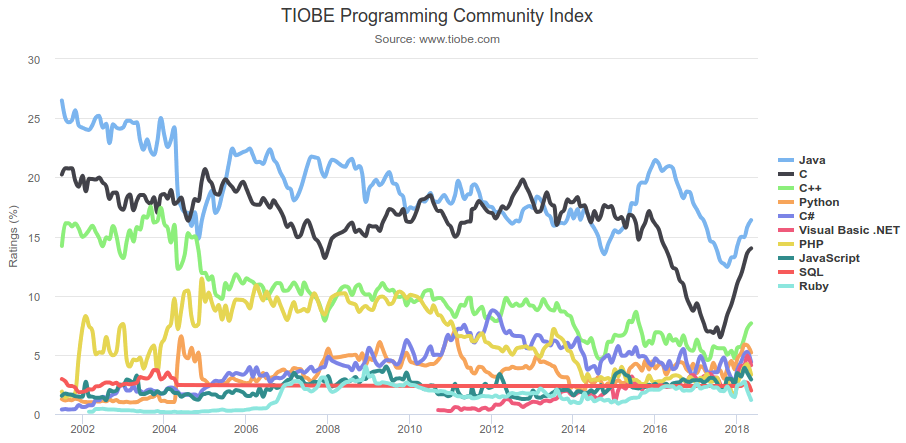
\includegraphics[width=12cm]{Tiobeindex}
		\caption{A programozási nyelvek népszerűségét mérő TIOBE index mozgása 2002-től 2015-ig. Ebben az időben az objektumorientált Java és a procedurális C vetélkedett egymással az első helyért} 
		\label{fig:TIOBE}
	\end{figure}
	
	Az 1990-es évek elején és közepén az objektumorientáció vált a programozás fő paradigmájává. Ezt támogatták azok az eszközök, amelyekkel az objektumorientált nyelvek elterjedhettek és népszerűvé váltak. Ezek közé tartozott a Visual FoxPro 3.0, a C++ és a Delphi. Dominanciáját az elterjedő vizuális felületek is erősítették, mivel ezek szerkesztéséhez az objektumorientált programozást támogatták. A szorosan összetartozó GUI könyvtár és objektumorientált nyelvre példa a Cocoa keretrendszer a Mac OS X operációs rendszer számára az Object-C nyelvhez. Az Object-C alapjában véve a C egy bővítése objektumorientált eszközökkel a Smalltalk alapján. Ezek az eszközök az eseményvezérelt programozást is elterjesztették.
	
	Az ETH Zürichnél Niklaus Wirth és társai vizsgálták az 1960-as évek óta használt adatabsztrakciót és a moduláris programozást. A Modula-2 (1978) mindkettőt magába foglalta. Továbbfejlesztése az Oberon újszerűen közelítette meg az objektumorientációt és az osztályokat.
	
	Több már korábban létező nyelvet bővítettek objektumorientált eszközökkel, például ezeket: Ada, BASIC, Fortran, Pascal, és COBOL. Ez kompatibilitási problémákat okozott és rontotta a karbantarthatóságot.
	
	Azóta számos olyan nyelv jelent meg, amelyek támogatják az objektumorientációt, de a procedurálisat is. Ezek közé tartozik a Python és a Ruby. A kereskedelmileg legfontosabb objektumorientált programozási nyelvek a Java , a C++, a C\# és a Visual Basic.NET (VB.NET). Ez utóbbiak eredetileg a Windowsra készültek, és mindegyik a maga módján használja az objektumorientációt. Támogatják a nyelvközi öröklést is, azaz az egyik nyelven írt osztályból lehet örökölni egy másik nyelven.
	
	\chapter{Irodalmak}
	\begin{itemize}
		\item Angster Erzsébet: Az objektumorientált tervezés és programozás alapjai (magánkiadás 1999; \href{https://hu.wikipedia.org/wiki/Speci\%C3\%A1lis:K\%C3\%B6nyvforr\%C3\%A1sok/9789636508180}{\textit{ISBN 978-963-650-818-0}} )
		\item Raffai Mária: Objektumtechnológia sorozat kötetei:
		\begin{itemize}
			\item Objektumok az üzleti modellezésben(\href{https://hu.wikipedia.org/wiki/Speci\%C3\%A1lis:K\%C3\%B6nyvforr\%C3\%A1sok/9639056286}{\textit{ISBN 963-9056-28-6}}; 2001)
			\item Egységesített megoldások a fejlesztésben(\href{https://hu.wikipedia.org/wiki/Speci\%C3\%A1lis:K\%C3\%B6nyvforr\%C3\%A1sok/9639056294}{\textit{ISBN 963-9056-29-4}}; 2001)
			\item Objektumorientált alkalmazásfejlesztés(\href{https://hu.wikipedia.org/wiki/Speci\%C3\%A1lis:K\%C3\%B6nyvforr\%C3\%A1sok/9639056316}{\textit{ISBN 963-9056-31-6}}; 2002)
			\item UML 2 modellező nyelvi kézikönyv(\href{https://hu.wikipedia.org/wiki/Speci\%C3\%A1lis:K\%C3\%B6nyvforr\%C3\%A1sok/9637692010}{\textit{ISBN 963-7692-01-0}}; 2005, 2007)
		\end{itemize}
		\item Erich Gamma, Richard Helm, Ralph Johnson, John Vlissides: Programtervezési minták (Kiskapu 2004; \href{https://hu.wikipedia.org/wiki/Speci\%C3\%A1lis:K\%C3\%B6nyvforr\%C3\%A1sok/9639301779}{\textit{ISBN 963-9301-77-9}})
		\item Raffai Mária: Információrendszer-fejlesztés (Novadat 1999; \href{https://hu.wikipedia.org/wiki/Speci\%C3\%A1lis:K\%C3\%B6nyvforr\%C3\%A1sok/9639056197}{\textit{ISBN 963-9056-19-7}})
	\end{itemize}
	
	\begin{thebibliography}{1}
		\bibitem{Kindler2011} \textsc{Kindler, E.:} \emph{,,Object-Oriented Simulation of systems with sophisticated control''}, 313–343. o, 2011, Kiadó: International Journal of General Systems.
		
		\bibitem{Mitchell} \textsc{John C. Mitchell:} \emph{Concepts in programming languages}, Cambridge University Press, 2003, ISBN 0-521-78098-5, p.278. Lists: Dynamic dispatch, abstraction, subtype polymorphism, and inheritance.
		
		\bibitem{Michael} \textsc{Michael Lee Scott:} \emph{Programming language pragmatics}, Edition 2, Morgan Kaufmann, 2006, ISBN 0-12-633951-1, p. 470. Lists encapsulation, inheritance, and dynamic dispatch.
		
		\bibitem{Booch} \textsc{Booch, Grady:} \emph{Software Engineering with Ada.} Addison Wesley, 220. o. (1986). ISBN 978-0805306088 „Perhaps the greatest strength of an object-oriented approach to development is that it offers a mechanism that captures a model of the real world.”
		
		\bibitem{Jacobsen} \textsc{Jacobsen, Ivar:} \emph{Object Oriented Software Engineering.} Addison-Wesley ACM Press, 43–69. o. (1992). ISBN 0-201-54435-0
		
		\bibitem{Neward} \textsc{Neward, Ted:} \emph{The Vietnam of Computer Science.} Interoperability Happens, 2006. június 26. [2006. július 4-i dátummal az eredetiből archiválva]. (Hozzáférés: 2010. június 2.)
		
		\bibitem{Holmevik} \textsc{Holmevik, Jan Rune:} \emph{,,Compiling Simula: A historical study of technological genesis.''} IEEE Annals of the History of Computing 16 (4), 1994, 25–37. o. DOI:10.1109/85.329756. (Hozzáférés ideje: 2018. március 3.)
	\end{thebibliography}
\end{document}